\documentclass{ximera}

\newcommand{\RR}{\mathbb R}
\renewcommand{\d}{\,d}
\newcommand{\dd}[2][]{\frac{d #1}{d #2}}
\renewcommand{\l}{\ell}
\newcommand{\ddx}{\frac{d}{dx}}
\newcommand{\dfn}{\textbf}
\newcommand{\eval}[1]{\bigg[ #1 \bigg]}


\outcome{Determine if a series converges using the alternating series test.}

\title[Dig-In:]{Remainders for alternating series}
\author{Jenny Sheldon and Jim Talamo}

\begin{document}
\begin{abstract}
There is a nice result for approximating the remainder of convergent alternating series. 
\end{abstract}
\maketitle

\section{Introduction}
In this section, we introduce a new type of series for which there is a nice result for the remainders.  Suppose that $\{a_n\}_{n=n_0}$ is a sequence of positive terms.  Then, we say that the series $\sum_{k=n_0}^{\infty} (-1)^k a_k$ is an \emph{alternating series}.

\begin{question}
Select all of the series below that are alternating series.

\begin{selectAll}
\choice[correct]{$\sum_{k=1}^{\infty} \frac{(-1)^k}{k}$}
\choice{$\sum_{k=1}^{\infty} \frac{(-1)^k}{\sin(k)}$}
\choice[correct]{$\sum_{k=1}^{\infty} \frac{(-1)^k}{k!}$}
\end{selectAll}
\end{question}

There is a nice result to test alternating series for convergence.

\begin{theorem}[Alternating Series Test]
Let $\{a_n\}_{n=n_0}$ be a sequence.  If

\begin{itemize}
\item $a_n \geq > 0$ eventually,
\item $a_{n+1} \leq a_n$ eventually, and
\item $\lim_{n \to \infty} a_n=0$, 
\end{itemize}

then, the alternating series $\sum_{k=n_0}^\infty (-1)^{k}a_k$ converges.
\end{theorem}

\begin{question}
Select all of the series below that converge by using the above test.

\begin{selectAll}
\choice[correct]{$\sum_{k=1}^{\infty} \frac{(-1)^k}{\sqrt{k}}$}
\choice{$\sum_{k=1}^{\infty} \frac{(-1)^k}{4}$}
\choice[correct]{$\sum_{k=1}^{\infty} \frac{(-1)^k}{k!}$}
\end{selectAll}
\end{question}

Note that this test gives us a way to show that certain alternating series converge, but it does not give us information about their corresponding values.  If we want to approximate such series, we must study their remainders!

  


%%%%%%%%%%%%%%%%%%%%%%%%%%%%%%%%%%%%%%%%%%%%%%%%%%%%%%%%%%%%%%%%%%%%%%

\section{Remainders for Alternating Series}
As usual we must establish that a series converges first before we begin to think about remainders.  Once we have established that an alternating series $\sum_{k=1}^{\infty} (-1)^k a_k$ converges, we have the usual decomposition.

\begin{image}
  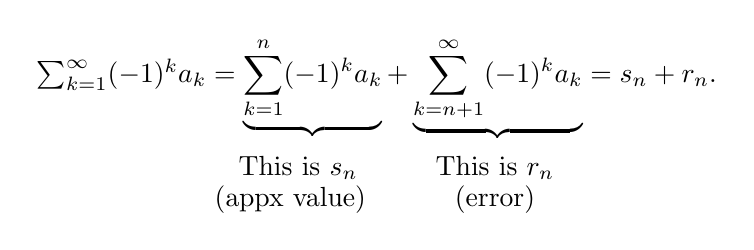
\begin{tikzpicture}
        \node at (0,0) {
          $ \sum_{k=1}^{\infty} (-1)^k a_k=\underbrace{\sum_{k=1}^{n}(-1)^k a_k}+ \underbrace{\sum_{k=n+1}^\infty (-1)^k a_k} = s_n+r_n$.};
        \node at (1.5,-1) {This is $r_n$};
           \node at (1.5,-1.4) {(error)};    
        \node at (-1,-1) {This is $s_n$ };
        \node at (-1.1,-1.4) {(appx value) };        
      \end{tikzpicture}
  \end{image}

As before, $s_n$ is the approximate value of the infinite series and $r_n$ is the error made when using this approximation.  While we cannot find an explicit formula for $s_n$, we have a good way to establish bounds on the error made when approximating $ \sum_{k=1}^{\infty} (-1)^k a_k$ by the finite sum $s_n= \sum_{k=1}^{n} (-1)^k a_k$, and this is made explicit in the theorem below.   

%%%%%%%%%%%%%%%%%%%%%%%%%%%%%%%%%%%%%%%%%%%%%%%%%%%%%%%%%%%%%%%%%
\begin{theorem}[Alternating Series Remainder Estimates]\index{alternating series remainder estimates}
Let $\{a_n\}_{n=n_0}$ be a sequence.  If

\begin{itemize}
\item $a_n \geq 0$,
\item $a_{n+1} \leq a_n$, and
\item $\lim_{n \to\infty} a_n=0$, 
\end{itemize}

then, we have the following estimate for the remainder.

\[
\big| r_n \big| \leq a_{n+1} \qquad \textrm{ for all } n \geq n_0,
\]
where $r_n = \sum_{k=n+1}^{\infty} a_k$.
\end{theorem}

Some insight into this test is given at the end of the section, which the curious reader may study should they wish.  In order to gain some practice with the test, let's work an example.

%%%%MOVE TO EXERCSIES%%%%%%%%%%%%%%%
%\begin{example}
%Consider the alternating geometric series $\sum_{k=0}^{\infty} (-1)^k \left(\frac{1}{2}\right)^k$.
%
%I. Compute $\sum_{k=0}^{\infty} (-1)^k \left(\frac{1}{2}\right)^k$.
%
%\begin{explanation}
%First, note that by using laws of exponents, $\sum_{k=0}^{\infty} (-1)^k \left(\frac{1}{2}\right)^k = \sum_{k=0}^{\infty}  \left(\frac{-1}{2}\right)^k$.   
%Hence, the geometric series $\sum_{k=0}^{\infty} (-1)^k \left(\frac{1}{2}\right)^k$ converges because $|r| = \frac{1}{2} \leq1$.
%
%
%When $r\leq1$, note that $\sum_{k=0}^{\infty} ar^k = \frac{a}{1-r}$.  Here, $r= -\frac{1}{2}$, so we find that $\sum_{k=0}^{\infty} (-1)^k \left(\frac{1}{2}\right)^k= \frac{2}{3}.$
%\end{explanation}
%
%II. Use the theorem above to obtain an estimate for the remainder if $s_4$ is used to approximate the series.  What do you notice?
%
%\begin{explanation}
%Since $\left\{\left(\frac{1}{2}\right)^k\right\}_{k=0}$ is decreasing and $\lim_{n \to \infty} \left(\frac{1}{2}\right)^n =0$, we can use the remainder results.  If we use $s_7$ to approximate  $\sum_{k=0}^{\infty} (-1)^k \left(\frac{1}{2}\right)^k$, we have $n=7$, and conclude
%
%\[
%|r_4| < a_5 = \left(\frac{1}{2}\right)^5 = \frac{1}{32}.
%\]
%
%We can explicitly compute $s_4$ by using the formula for partial sums for geometric series or by hand.
%
%\[
%s_4 = 1-\frac{1}{2}+\frac{1}{4}-\frac{1}{8}+\frac{1}{16} = \frac{11}{16}.
%\]
%
%We note that to five decimal places, we have the following.
%
%\begin{itemize}
%\item The error bound from the theorem is $|r_4| < \frac{1}{32} = .03125$.
%\item The approximate value of the series $\sum_{k=0}^{\infty} (-1)^k \left(\frac{1}{2}\right)^k$ is $s_4 = \frac{11}{16} = .68750$.
%\item The actual value of the series $\sum_{k=0}^{\infty} (-1)^k \left(\frac{1}{2}\right)^k$ is $\frac{2}{3} \approx .66667$.
%\end{itemize}
%
%Thus, $s_4$ is actually within $.02083$ of the actual value of $\sum_{k=0}^{\infty} (-1)^k \left(\frac{1}{2}\right)^k$; $s_4$ is thus within the $.03125$ of the actual value of $\sum_{k=0}^{\infty} (-1)^k \left(\frac{1}{2}\right)^k$ guaranteed by the remainder result.
%
%\end{explanation}
%\end{example}
%
%In the above example, we could compute the exact value of the series in question, so the remainder result could be verified explicitly.  In the next example, the exact value of the series is not known, but we can approximate as closely as we want.
\begin{example}
Consider the series $\sum_{k=1}^\infty \frac{(-1)^k}{k^2}$.  Give an upper bound for the absolute value of the error involved with using $s_8$ in place of the exact value of the series, which we call $S$.

\begin{explanation}
First, notice that the series is a convergent alternating series - so it makes sense to even ask the question in the first place!

Second, our error estimate is simply the next term of the series.  In particular, 
\begin{align*}
\vert r_8 \vert &< a_{\answer[given]{9}}\\
 &= \answer[given]{1/81}.
\end{align*}
\end{explanation}

\end{example}

Simple enough!  Let's see if our other typical question presents any additional trouble.

\begin{example}
How many terms of the series $\sum_{k=1}^{\infty}\frac{(-1)^k}{k^2}$ do we need to add in order to guarantee that the estimate $s_n$ is within $0.01$ of the actual sum $S$?
\begin{explanation}
Here we are looking for a value of $n$ after which we are guaranteed small enough error.  Again, we will use the Alternating Series Test to answer this question.

We know that
\[
\vert r_n \vert \leq a_{\answer[given]{n+1}},
\]
so if we can force our upper bound to be less than $0.01$, then the size of the remainder can be no larger.  Now
\begin{align*}
   a_{\answer[given]{n+1}} &\leq 0.01 \\
   \frac{1}{ \answer[given]{(n+1)^2}} & \leq \frac{1}{100}
\end{align*}
is satisfied for 
\[
100 \leq \answer[given]{(n+1)^2}.
\]
Taking the square root of both sides, we see that we need
\[
10 \leq \answer[given]{n+1}
\]
or
\[
n \geq \answer[given]{9}.
\]
In other words, when $n \geq \answer[given]{9}$, we have
\[
\vert r_n \vert \leq a_{n+1} \leq 0.01.
\]
\end{explanation}
\end{example}

\begin{remark}
Note that the above guarantees that for any integer $N>n_0$, the term $s_N$ will approximate the series $\sum_{k=1}^{\infty} a_k$ with an error of magnitude no greater than $a_{n+1}$.  Since we are now working with series which have both positive and negative terms, we have switched to talking about the size of the error rather than its actual value.  The remainder itself could be positive or negative, depending on our series and the chosen value of $n$.  The size, or absolute value, of the remainder gives us the information we usually want in practice -- how far are we from the sum?  But if an application problem is asking you whether the partial sum is above or below the sum, you can now answer that question as well!
\end{remark}
%MOVE TO EXERCISES

%\begin{example}
%Consider the alternating series $\sum_{k=1}^{\infty} \frac{(-1)^k}{k^3}$.
%
%I. Find a value for $N$ so $s_N$ approximates $\sum_{k=1}^{\infty} \frac{(-1)^k}{k^3}$ to within $.0001$ of its actual value.
%
%\begin{explanation}
%Check for yourself that $\sum_{k=1}^{\infty} \frac{(-1)^k}{k^3}$ satisfies the criteria for the remainder result for alternating series to hold before reading on.
%
%To find a value for $N$ so $s_N$ approximates $\sum_{k=1}^{\infty} \frac{(-1)^k}{k^3}$ to within $.0001$ of its actual value, we can find $N$ so $\big|r_N\big| \leq .0001$.  Since we have an explicit formula $a_n = \frac{1}{n^3}$ and that $\big|r_N\big| \leq a_{N+1}$, we can set $a_{N+1} \leq .0001$ (so $|r_N|$ will be less than $.0001$ by transitivity).
%
%\begin{align*}
%a_{N+1} = \frac{1}{\answer{\left(N+1\right)^3}} &\leq .0001 \\
%1 &\leq  .0001 (N+1)^3 \\
%\answer{10000} &\leq (N+1)^3 \\
%21.54 &\leq N+1 \qquad  \textrm{ (to two decimal places) }\\
%20.54 &\leq N \\
%\end{align*}
%
%We should thus use $N =$  \wordChoice{\choice{$20$}\choice[correct]{$21$}}.
%\end{explanation}
%
%II. Using technology, compute $\sum_{k=1}^{\infty} \frac{(-1)^k}{k^3}$ to within $.0001$.
%
%\begin{explanation}
% We can thus approximate $\sum_{k=1}^{\infty} \frac{(-1)^k}{k^3}$ by using \wordChoice{\choice{$s_{20}$}\choice[correct]{$s_{21}$}}.  While this would be tedious to do by hand, technology can compute this sum quickly to find 
%
%\[
%\sum_{k=1}^{21} \frac{(-1)^k}{k^3} \approx -.90159.
%\]
%
%\begin{remark}
%By noting that when $k=21$, the term $\frac{(-1)^k}{k^3}$ is negative, we see that $s_{21}$ will actually be an underestimate.  We may thus conclude that $-.90159 \leq \sum_{k=1}^{\infty} \frac{(-1)^k}{k^3} \leq -.90159+.0001$.
%\end{remark}
%
%\end{explanation}
%
%III. Using technology, it can be shown that $\sum_{k=1}^{100000} \frac{(-1)^k}{k^3} = -.9015426774$ to ten decimal places.  Using the remainder result, how far off from the exact value of the series $\sum_{k=1}^{100000} \frac{(-1)^k}{k^3}$ could this be?
%
%
%\begin{explanation}
%Here, we have used $s_{100000}$ to approximate the value of the series.  The remainder result tells us that the error $r_{100000}$ made in this approximation can be no worse than $a_{100001}$; i.e.
%
%\[
%\big|r_{100000}\big| \leq \frac{1}{(100001)^3}. 
%\]
%
%Noting that $\frac{1}{(100001)^3} = 9.9997 \times 10^{-16}$, we see that the approximation given above corresponds with the actual value of the series to the ten decimal places listed.
%
%\end{explanation}
%\end{example}

Finally, let's consider one more problem.
\begin{question}
Determine if there is a value for $N$ so $\sum_{k=1}^{N} (-1)^k \cdot \frac{k+2}{2k+1}$ is within $.01$ of the value of $\sum_{k=1}^{N} (-1)^k \cdot \frac{k+2}{2k+1}$.  If there is such a value, give one possibility for it.

\begin{multipleChoice}
\choice[correct]{There is no such value for $N$ since the series $\sum_{k=1}^{N} (-1)^k \cdot \frac{k+2}{2k+1}$ diverges.}
\choice{There is such a value for $N$.}
\end{multipleChoice}

\begin{feedback}
Note that before we try to approximate the value of a series, we must first determine that it converges (so it actually \emph{has} a value).  Here, note that $\lim_{n \to \infty} \frac{n+2}{2n+1} = \frac{1}{2}$, so $\lim_{n \to \infty} (-1)^n \cdot \frac{n+2}{2n+1}$ does not exist, and hence $\sum_{k=1}^{N} (-1)^k \cdot \frac{k+2}{2k+1}$ diverges by the divergence test.
\end{feedback}
\end{question}

\section{Summary}

When $\{a_n\}_{n = n_0}$ is a decreasing sequence of positive term, we will approximate $\sum_{k=n_0}^{\infty} a_k$ by the finite sum $s_n =\sum_{k=n_0}^{n} a_k$.  Generally, adding more and more terms of a convergent series should generally get you closer to the actual sum!
Indeed, we have a nice bound for the remainder:

\[ \textrm{magnitude of error} = |r_n| \leq a_{n+1}.\]  

We can use to approximate the series to any degree of accuracy as we want!




%%%%%%%%%%%%%%%%%%%%%%%%%%%%%%%%%%%%%%%%%%%%%%%%%%%%%%%%%%%%%%%%%

\section{Why the Alternating Series Test Works}

Recall the Alternating Series Test Estimate, which is listed below.

\begin{quote}
Let $\{a_n\}_{n=n_0}$ be a sequence.  If

\begin{itemize}
\item $a_n \geq 0$,
\item $a_{n+1} \leq a_n$, and
\item $\lim_{n \to\infty} a_n=0$, 
\end{itemize}

then, we have the following estimate for the remainder.

\[
\big| r_n \big| \leq a_{n+1} \qquad \textrm{ for all } n \geq n_0,
\]
where $r_n = \sum_{k=n+1}^{\infty} a_k$.
\end{quote}


Let's explore this result pictorially for a general alternating series.

\begin{model}
Let's begin with a convergent alternating series $\sum_{k=0}^{\infty} (-1)^k a_k$ for which the alternating series test applies.  For the sake of argument, we make the following conventions to begin the example.

\begin{itemize}
\item $a_n > 0$ for every $n \geq 0$. 
\item $\{a_n\}_{n=0}$ is strictly decreasing immediately; that is $a_{n+1} < a_n$ for every $n \geq 0$. 
\item $\lim_{n\to\infty} a_n= 0$ (not really an assumption since $\sum_{k=0}^{\infty} (-1)^k a_k$ converges).
\item The value of the convergent series $\sum_{k=0}^{\infty} (-1)^k a_k$ is the number $S$.
\end{itemize}

Let's plot the terms of two sequences : $\{a_n\}_{n=0}$, which consists of \emph{positive} terms and the  sequence of partial sums $\{s_n\}_{n=0}$ for the alternating series $\sum_{k=0}^{\infty} (-1)^k a_k$.  We first start with the plot of $\{a_n\}_{n=0}$.

\begin{image}
\begin{tikzpicture}
	\begin{axis}[
            domain=.8:6,xmin=-.5,xmax=8.5,ymin=-.5,ymax=10,
            width=4in,
            height=2in,
            axis lines =middle, xlabel=$n$, ylabel=$a_n$,
            xtick={1,2,...,7},
            xticklabels={$1$,$2$,$3$,$4$,$\ldots$,$n$, $n+1$},
            ytick={11},
            every axis y label/.style={at=(current axis.above origin),anchor=south},
            every axis x label/.style={at=(current axis.right of origin),anchor=west},
            clip=false,
            %axis on top,
          ]
       
          \addplot[color=penColor,fill=penColor,only marks,mark=*,ultra thick] coordinates{(0,8)};  %% closed hole          
          \addplot[color=penColor,fill=penColor,only marks,mark=*,ultra thick] coordinates{(1,6)};  %% closed hole    
          \addplot[color=penColor,fill=penColor,only marks,mark=*,ultra thick] coordinates{(2,4.5)};  %% closed hole 
          \addplot[color=penColor,fill=penColor,only marks,mark=*,ultra thick] coordinates{(3,3.5)};  %% closed hole  
          \addplot[color=penColor,fill=penColor,only marks,mark=*,ultra thick] coordinates{(4,2.5)};  %% closed hole   
          
          \addplot[color=penColor,fill=penColor,only marks,mark=*,ultra thick] coordinates{(6,1.3)};  %% closed hole  
          \addplot[color=penColor,fill=penColor,only marks,mark=*,ultra thick] coordinates{(7,1)};  %% closed hole  

%%%%Labels
        \node[above right] at (axis cs:0,8) {\small{$a_0$}};
        \node[above right] at (axis cs:1,6.5) {\small{$a_1$}};
        \node[above right] at (axis cs:2,4.5) {\small{$a_2$}};
        \node[above right] at (axis cs:3,3.5) {\small{$a_3$}};
        \node[above right] at (axis cs:4,2.5) {\small{$a_4$}};
        \node[above right] at (axis cs:6,1.3) {\small{$a_n$}};
        \node[above right] at (axis cs:7,1) {\small{$a_{n+1}$}};
        \node at (axis cs:5,2) {$\ldots$};                            
        \end{axis}
\end{tikzpicture}
\end{image}

%%%%%%%

We now plot the terms in the series $\sum_{k=0}^{\infty} (-1)^ka _k$.  Note that when written out, the sum in question is

\[
a_0-a_1+a_2-a_3+\ldots
\]
That is, we alternate between adding and subtracting terms in the sequence $\{a_n\}_{n=0}$.  

\begin{image}
\begin{tikzpicture}
	\begin{axis}[
            domain=.8:6,xmin=-.5,xmax=8.5,ymin=-.5,ymax=10,
            width=4in,
            height=2in,
            axis lines =middle, xlabel=$n$, ylabel=$a_n$,
            xtick={1,2,...,7},
            xticklabels={$1$,$2$,$3$,$4$,$\ldots$,$n$, $n+1$},
            ytick={11},
            every axis y label/.style={at=(current axis.above origin),anchor=south},
            every axis x label/.style={at=(current axis.right of origin),anchor=west},
            clip=false,
            %axis on top,
          ]
          \addplot[color=penColor,fill=penColor,only marks,mark=*,ultra thick] coordinates{(0,8)};  %% closed hole           
          \addplot[color=penColor,fill=penColor,only marks,mark=*,ultra thick] coordinates{(1,2)};  %% closed hole          
          \addplot[color=penColor,fill=penColor,only marks,mark=*,ultra thick] coordinates{(2,7)};  %% closed hole 
          \addplot[color=penColor,fill=penColor,only marks,mark=*,ultra thick] coordinates{(3,2.7)};  %% closed hole  
          \addplot[color=penColor,fill=penColor,only marks,mark=*,ultra thick] coordinates{(4,6)};  %% closed hole   
          
          \addplot[color=penColor,fill=penColor,only marks,mark=*,ultra thick] coordinates{(6,5)};  %% closed hole  
          \addplot[color=penColor,fill=penColor,only marks,mark=*,ultra thick] coordinates{(7,3.2)};  %% closed hole  

%%%%Labels
        \node[above left] at (axis cs:0,8) {\small{$s_0$}};
        \node[above left] at (axis cs:1,2) {\small{$s_1$}};
        \node[above left] at (axis cs:2,7) {\small{$s_2$}};
        \node[above left] at (axis cs:3,2.7) {\small{$s_3$}};
        \node[above left] at (axis cs:4,6) {\small{$s_4$}};
        \node[above left] at (axis cs:6,5) {\small{$s_n$}};
        \node[below left] at (axis cs:7,3.2) {\small{$s_{n+1}$}};
        \node at (axis cs:5,2) {$\ldots$};   
        
\node at (axis cs: -.5,4) {$S$};        
	\addplot [draw=penColor, fill = penColor,dashed] plot coordinates {(-.2,4) (8.5,4)};           
	
\draw[<->] (axis cs: .2,8) -- (axis cs:.2, 4) node[pos=0.5, right] {$r_0$};	
\draw[<->] (axis cs: 1.2,2) -- (axis cs:1.2, 4) node[pos=0.5, right] {$r_1$};	
\draw[<->] (axis cs: 2.2,7) -- (axis cs:2.2, 4) node[pos=0.5, right] {$r_2$};	
\draw[<->] (axis cs: 3.2,2.7) -- (axis cs:3.2, 4) node[pos=0.5, right] {$r_3$};
\draw[<->] (axis cs: 4.2,6) -- (axis cs:4.2, 4) node[pos=0.5, right] {$r_4$};		
\draw[<->] (axis cs: 6.2,5) -- (axis cs:6.2, 4) node[pos=0.5, right] {$r_n$};	
	
	      
        \end{axis}
\end{tikzpicture}
\end{image}

Note that in the above picture, the term $r_n$ corresponding to the error made when we use $s_n$ to approximate the infinite series is the difference between the actual value of the series, and $s_n$. 

We now note the following.  For odd indices $n$, we have (from the picture) the relationship below. 
\[
s_1 > s_3 > s_5 > s_7 > \dots > S,
\]
By the same logic about the relative sizes of the terms, we have for even $n$ that
\[
s_2 < s_4 < s_6 < s_8 < \dots < S.
\]


Now, we can think of the remainder $r_n$ as the difference between $S$ and $s_n$ at any stage, or that
\begin{image}
  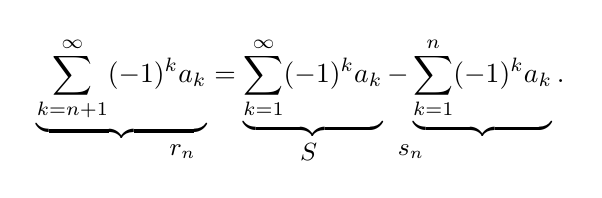
\begin{tikzpicture}
        \node at (0,0) {
           $\underbrace{\sum \limits_{k=n+1}^\infty (-1)^k a_k}  = \underbrace{\sum \limits_{k=1}^\infty (-1)^k a_k} - \underbrace{\sum \limits_{k=1}^n (-1)^k a_k}. $ 
           };
        \node at (-1.5, -.8) {\small{$r_n$}};
        \node at (0.1,-.8) {\small{$S$}};
        \node at (1.4, -.8) {\small{$s_n$}};
      \end{tikzpicture}
  \end{image}
When $n$ is even, $s_n > S$.  But then $n+1$ is odd, meaning that $s_{n+1} < S$.  To get from $s_n$ to $s_{n+1}$, we subtract $s_n - a_{n+1}$.  But this subtraction takes us from a number greater than $S$ to a number less than $S$.  In other words, the distance between $S$ and $s_n$ is less than $a_{n+1}$.  In symbols, 
\[
\vert S - s_n \vert < a_{n+1}.
\]
Similarly, if $n$ is odd, then $n+1$ is even, so that $s_n < S$ and $s_{n+1} > S$.  Again, since $s_{n+1} = s_n + a_{n+1}$, the distance between $S$ and $s_n$ is less that $a_{n+1}$.  But this distance is precisely the absolute value of $r_n$.

\end{model}

Of course, if $a_1$ is negative, we have the same behavior, except the odd partial sums are increasing and the even ones are decreasing.  Try it out with an example if you are skeptical!  We can now state the general result for approximating alternating series.


%
%\begin{remark}
%Note that while the actual alternating series test requires that the terms $a_k$ in the series $\sum_{k=n_0} (-1)^k a_k$ or $\sum_{k=n_0} (-1)^{k+1} a_k$ eventually be positive and decreasing, the remainder results \emph{require} this for all terms; that is $a_n$ must be positive and $a_{n+1} \leq a_n$ for all $n \geq n_0$.  If this is not the case, care must be taken when constructing the estimates.  Details are left for the curious reader to ponder.
%\end{remark}



%Let's see the details of the test in the context of an example.
%
%\begin{model}
%Consider the alternating harmonic series $\sum_{k=1}^{\infty} \frac{(-1)^k}{k}$.  Here, $a_n = \frac{1}{n}$, and the reader can verify that the series meets the hypothesis for the alternating series test.  To develop some intuition about the error made when we approximate the infinite series by adding only finitely many of its terms, let's write out some of its terms.
%
%\[
%\sum_{k=1}^{\infty} \frac{(-1)^k}{k} = -1+\frac{1}{2}-\frac{1}{3}+\frac{1}{4}-\frac{1}{5}+\frac{1}{6}-\frac{1}{7} + \ldots
%\]
%
%Now, let's say we want to approximate the infinite series with $s_2$.
%
%\begin{image}
%  \begin{tikzpicture}
%        \node at (0,0) {
%          $\sum_{k=1}^{\infty} \frac{(-1)^k}{k}=\underbrace{-1+\frac{1}{2}}-\frac{1}{3}+ \underbrace{\left[\frac{1}{4}-\frac{1}{5}\right]}+\underbrace{\left[\frac{1}{6}-\frac{1}{7}\right]} + \ldots$};
%        \node at (.9,-1) { positive};
%         \node at (2.6,-1) { positive};      
%        \node at (-1.4,-.8) { $s_2$};
%        
%      \end{tikzpicture}
%  \end{image}
%  
%  Note that each pair of terms we've enclose in brackets is \wordChoice{\choice[correct]{positive}\choice{negative}}, which means that
%  
%  \[
%  \sum_{k=1}^{\infty} \frac{(-1)^k}{k} \geq -1+\frac{1}{2}-\frac{1}{3} = s_2 -a_3
%  \]
%  
%  Similarly, had we used $s_3$ for the approximation, we could obtain an overestimate for the value of the series.
%  
%  \begin{image}
%  \begin{tikzpicture}
%        \node at (0,0) {
%          $\sum_{k=1}^{\infty} \frac{(-1)^k}{k}=\underbrace{-1+\frac{1}{2}-\frac{1}{3}}+ \frac{1}{4}+\underbrace{\left[-\frac{1}{5}+\frac{1}{6}\right]}+\underbrace{\left[-\frac{1}{7} +\frac{1}{8}\right]} + \ldots$};
%        \node at (1.1,-1) { negative};
%         \node at (3.1,-1) { negative};      
%        \node at (-1.7,-.8) { $s_3$};
%        
%      \end{tikzpicture}
%  \end{image}
%  
%    Note that each pair of terms we've enclose in brackets is \wordChoice{\choice{positive}\choice[correct]{negative}}, which means that
%  
%  \[
%  \sum_{k=1}^{\infty} \frac{(-1)^k}{k} \leq -1+\frac{1}{2}-\frac{1}{3} +\frac{1}{4} = s_3 -a_4
%  \]
%  
%Note that since we can split the convergent series up as
%
%\[
%\sum_{k=1}^{\infty} \frac{(-1)^k}{k} = s_n +r_n,
%\]
%We can see in both cases that the magnitude of the error is bounded above by the magnitude of the next term in the series; that is 
%
%\[\big| r_n \big| \leq a_{n+1}.\]
%
%We can repeat this construction by using $s_n$ for an unspecified value for $n$ and arrive at the conclusion above.  
%\end{model}
%
%\begin{remark}
%Note that while the actual alternating series test requires that the terms $a_k$ in the series $\sum_{k=n_0} (-1)^k a_k$ or $\sum_{k=n_0} (-1)^{k+1} a_k$ eventually be positive and decreasing, the remainder results \emph{require} this for all terms; that is $a_n$ must be positive and $a_{n+1} \geq a_n$ for all $n \geq n_0$.  If this is not the case, care must be taken when constructing the estimates.  Details are left for the curious reader to ponder.
%\end{remark}
%
%
%
%
%
%We hope that the curious reader explores that a similar argument can be made for series that meet the assumptions of the alternating series remainder test.  
%
%\textbf{ADD JENNY'S PICTURE?}
%

\end{document}
